\chapter{Polymers}\label{ch:g12:polymers}

A fleece jacket can be spun from melted drink bottles; a climbing rope is
made of nylon; this page is cellulose, made by trees. All three are
\omterm{def:g12:polymers:polymer}{polymers}: \omterm{def:g7:atoms-and-molecules:molecule}{molecules} thousands of \omterm{def:g7:atoms-and-molecules:atom}{atoms} long, built by repeating one small
unit again and again. Their properties --- soft or rigid, elastic or
brittle, meltable or not --- come less from the \omterm{def:g7:atoms-and-molecules:atom}{atoms} they contain than
from the way their long chains are arranged.

\begin{recall}
\omterm{def:g8:plastics:plastic}{Plastics} are made of very long \omterm{def:g7:atoms-and-molecules:molecule}{molecules}; \omterm{def:g8:plastics:thermoplastic}{thermoplastics} soften on
heating, \omterm{def:g8:plastics:thermoplastic}{thermosets} do not (\cref{ch:g8:plastics}). \omterm{def:g11:functional-groups:alcohol}{Alcohol}, acid, \omterm{def:g11:functional-groups:carboxylic-acid}{ester},
\omterm{def:g11:functional-groups:amine}{amine} and \omterm{def:g11:functional-groups:amine}{amide} groups (\cref{ch:g11:functional-groups}). An addition
joins two \omterm{def:g7:atoms-and-molecules:molecule}{molecules} into one without losing any \omterm{def:g7:atoms-and-molecules:atom}{atom}
(\cref{ch:g12:curly-arrows}).
\end{recall}

\begin{omfigure}
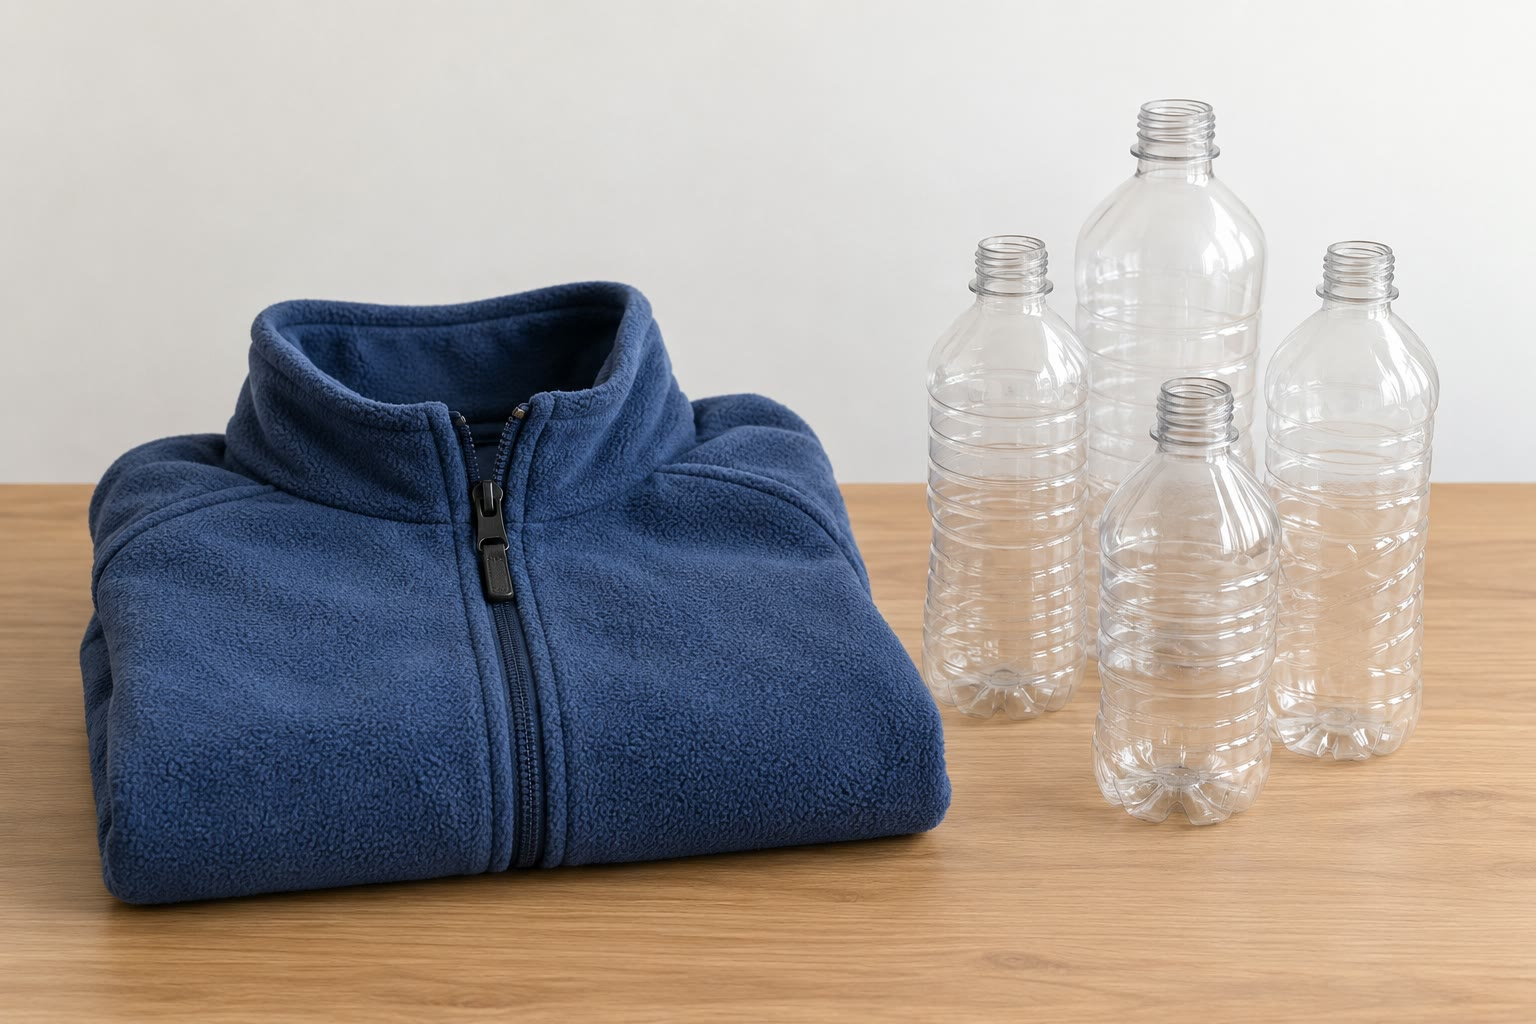
\includegraphics[width=0.45\linewidth]{images/book1/ai/g12-fleece-bottles.jpg}

{\small Used drink bottles and a fleece jacket: the same \omterm{def:g12:polymers:polymer}{polymer}, in two
shapes.}
\end{omfigure}

\section{Monomers, polymers, repeat units}

\begin{definition}[Polymer, monomer, polymerisation]\label{def:g12:polymers:polymer}
A \emph{polymer}\index{polymer} is a substance made of very large
\omterm{def:g7:atoms-and-molecules:molecule}{molecules}, the macromolecules, each built from many small units bonded
one after the other. The small \omterm{def:g7:atoms-and-molecules:molecule}{molecules} from which it is made are its
\emph{monomers}\index{monomer}; the reaction that joins them is a
\emph{polymerisation}\index{polymerisation}.
\end{definition}

\begin{definition}[Repeat unit, degree of polymerisation]\label{def:g12:polymers:repeat-unit}
The \emph{repeat unit}\index{repeat unit} of a \omterm{def:g12:polymers:polymer}{polymer} is the smallest
group of \omterm{def:g7:atoms-and-molecules:atom}{atoms} whose repetition gives the chain; it is written between
brackets with an index $n$. The number $n$ of repeat units in a chain is
its \emph{degree of polymerisation}\index{degree of polymerisation}.
\end{definition}

\begin{omfigure}
\[
  n\;\ce{CH2=CH2}
  \quad\longrightarrow\quad
  \chemfig{-[@{op1,.75}]CH_2-CH_2-[@{cl1,0.25}]}
  \polymerdelim[height=6pt, depth=6pt, indice=n]{op1}{cl1}
\]

{\small The \omterm{def:g12:polymers:polymer}{polymerisation} of ethene: $n$ \omterm{def:g7:atoms-and-molecules:molecule}{molecules} of \omterm{def:g12:polymers:polymer}{monomer} give one
chain of polyethene, whose \omterm{def:g12:polymers:repeat-unit}{repeat unit} \ce{-CH2-CH2-} is written between
brackets.}
\end{omfigure}

\begin{proposition}[Molar mass of a polymer]\label{prop:g12:polymers:molar-mass}
A chain of \omterm{def:g12:polymers:repeat-unit}{degree of polymerisation} $n$ has a \omterm{def:g10:the-mole:molar-mass}{molar mass}
\[
  M(\text{polymer}) \approx n \times M(\text{repeat unit}) ,
\]
the two ends of the chain being negligible for large $n$.
\end{proposition}

\begin{proof}
The chain is $n$ \omterm{def:g12:polymers:repeat-unit}{repeat units} plus two end groups of a few \omterm{def:g7:atoms-and-molecules:atom}{atoms} each;
for $n$ in the thousands, the end groups weigh less than a thousandth of
the whole.
\end{proof}

\begin{example}[A polyethene chain]\label{ex:g12:polymers:pe}
% ledger: aw:C, aw:H
A chain of polyethene of \omterm{def:g10:the-mole:molar-mass}{molar mass} \qty{280000}{g/mol} has
$n = 280000/28.0 = 10000$ \omterm{def:g12:polymers:repeat-unit}{repeat units}, so twenty thousand carbon \omterm{def:g7:atoms-and-molecules:atom}{atoms}
in a row. In a real sample the chains do not all have the same length:
$n$ is an average.
\end{example}

\section{Addition polymers}

\begin{definition}[Addition polymer, condensation polymer]\label{def:g12:polymers:addition-polymer}
An \emph{addition polymer}\index{addition polymer} forms by additions
of \omterm{def:g12:polymers:polymer}{monomers} carrying a \ce{C=C} \omterm{def:g10:lewis-and-shape:multiple-bond}{double bond}, with no other product: its
\omterm{def:g12:polymers:repeat-unit}{repeat unit} has the same \omterm{def:g7:atoms-and-molecules:atom}{atoms} as the \omterm{def:g12:polymers:polymer}{monomer}. A \emph{condensation
polymer}\index{condensation polymer} forms by reactions between two
\omterm{def:g11:functional-groups:functional-group}{functional groups} that join two \omterm{def:g12:polymers:polymer}{monomers} and release a small \omterm{def:g7:atoms-and-molecules:molecule}{molecule},
usually water, at each link.
\end{definition}

\begin{omfigure}
\footnotesize
\renewcommand{\arraystretch}{1.5}
\begin{tabular}{l l l l}
\hline
\omterm{def:g12:polymers:polymer}{monomer} & \omterm{def:g12:polymers:polymer}{polymer} & \omterm{def:g12:polymers:repeat-unit}{repeat unit} & uses \\
\hline
ethene \ce{CH2=CH2} & polyethene (PE) & \ce{-CH2-CH2-} & bags, bottles \\
chloroethene \ce{CH2=CHCl} & poly(vinyl chloride) (PVC) & \ce{-CH2-CHCl-} & pipes, frames \\
phenylethene \ce{CH2=CH-C6H5} & polystyrene (PS) & \ce{-CH2-CH(C6H5)-} & cups, foam \\
tetrafluoroethene \ce{CF2=CF2} & PTFE & \ce{-CF2-CF2-} & non-stick pans \\
\hline
\end{tabular}\par\medskip

{\small Four \omterm{def:g12:polymers:addition-polymer}{addition polymers}. In each, the \omterm{def:g10:lewis-and-shape:multiple-bond}{double bond} of the \omterm{def:g12:polymers:polymer}{monomer}
opens, and its two carbons join the chain.}
\end{omfigure}

\begin{method}[Finding the monomer from a polymer]\label{met:g12:polymers:monomer}
\begin{enumerate}
  \item Find the \omterm{def:g12:polymers:repeat-unit}{repeat unit}: the smallest group whose repetition gives
        the chain.
  \item If the main chain holds only carbon \omterm{def:g7:atoms-and-molecules:atom}{atoms}, it is an \omterm{def:g12:polymers:addition-polymer}{addition
        polymer}: put back a \omterm{def:g10:lewis-and-shape:multiple-bond}{double bond} between the two carbons of the
        \omterm{def:g12:polymers:repeat-unit}{repeat unit}'s main chain. That is the \omterm{def:g12:polymers:polymer}{monomer}.
  \item If the main chain holds \omterm{def:g11:functional-groups:carboxylic-acid}{ester} or \omterm{def:g11:functional-groups:amine}{amide} links, it is a
        \omterm{def:g12:polymers:addition-polymer}{condensation polymer}: cut each link, and give back to each side
        the \omterm{def:g7:atoms-and-molecules:atom}{atoms} of the small \omterm{def:g7:atoms-and-molecules:molecule}{molecule} released (\ce{-OH} to the
        \ce{C=O}, \ce{-H} to the \ce{O} or \ce{N}). Those are the
        \omterm{def:g12:polymers:polymer}{monomers}.
\end{enumerate}
\end{method}

\begin{example}[The monomer of PVC]\label{ex:g12:polymers:pvc}
The chain \ce{-CH2-CHCl-CH2-CHCl-CH2-CHCl-} repeats \ce{-CH2-CHCl-}; it
holds only carbons in its main chain, so the \omterm{def:g12:polymers:polymer}{monomer} is
\ce{CH2=CHCl}, chloroethene.
\end{example}

\section{Condensation polymers}

A \omterm{def:g12:polymers:polymer}{monomer} with one reactive group can bond only once: it ends a chain.
To build a chain by condensation, each \omterm{def:g12:polymers:polymer}{monomer} needs two groups, one at
each end.

\begin{example}[PET, a polyester]\label{ex:g12:polymers:pet}
% ledger: aw:C, aw:H, aw:O
Ethane-1,2-diol, \ce{HO-CH2-CH2-OH}, carries two \omterm{def:g11:functional-groups:alcohol}{alcohol} groups;
benzene-1,4-dicarboxylic acid, \ce{HOOC-C6H4-COOH}, two acid groups. Each
acid group forms an \omterm{def:g11:functional-groups:carboxylic-acid}{ester} with an \omterm{def:g11:functional-groups:alcohol}{alcohol} group and releases water: the
chain grows from both ends. The \omterm{def:g12:polymers:polymer}{polymer} is poly(ethylene terephthalate),
PET, the material of drink bottles and of polyester fibres. Its \omterm{def:g12:polymers:repeat-unit}{repeat
unit}, \ce{C10H8O4}, has a \omterm{def:g10:the-mole:molar-mass}{molar mass} of \qty{192.0}{g/mol}, that is the
two \omterm{def:g12:polymers:polymer}{monomers} ($62.0 + 166.0$) minus two \omterm{def:g7:atoms-and-molecules:molecule}{molecules} of water ($36.0$).
\end{example}

\begin{omfigure}
\setchemfig{atom sep=1.9em}
\chemfig{HO-CH_2-CH_2-OH}
\quad $+$ \quad
\chemfig{HO-C(=[2]O)-*6(-=-(-C(=[2]O)-OH)=-=)}

\medskip
$\longrightarrow$\quad
\chemfig{-[@{op2,.75}]O-CH_2-CH_2-O-C(=[2]O)-*6(-=-(-C(=[2]O)-[@{cl2,0.25}])=-=)}
\polymerdelim[height=20pt, depth=6pt, indice=n]{op2}{cl2}
\quad $+\ 2n\ \ce{H2O}$

{\small PET from its two \omterm{def:g12:polymers:polymer}{monomers}: each \omterm{def:g11:functional-groups:carboxylic-acid}{ester} link (the \ce{-CO-O-}
groups) releases one \omterm{def:g7:atoms-and-molecules:molecule}{molecule} of water.}
\end{omfigure}

\begin{example}[Nylon-6,6, a polyamide]\label{ex:g12:polymers:nylon}
Hexane-1,6-diamine, \ce{H2N-(CH2)6-NH2}, and hexanedioic acid,
\ce{HOOC-(CH2)4-COOH}, join by \omterm{def:g11:functional-groups:amine}{amide} links, each releasing one \omterm{def:g7:atoms-and-molecules:molecule}{molecule}
of water:
\[
  \cdots\ce{-NH-(CH2)6-NH-CO-(CH2)4-CO-}\cdots
\]
The two sixes in the name count the carbon \omterm{def:g7:atoms-and-molecules:atom}{atoms} of each \omterm{def:g12:polymers:polymer}{monomer}. The
\omterm{def:g11:functional-groups:amine}{amide} links of neighbouring chains attract each other by \omterm{def:g11:polarity-and-cohesion:hydrogen-bond}{hydrogen bonds},
which makes nylon fibres strong.
\end{example}

\begin{history}[Carothers and nylon]
% ledger: hist:polyamides-1934, hist:nylon-production-1939
The chemist Wallace Carothers, who led a research laboratory of a
chemical company, set out to prove that \omterm{def:g12:polymers:polymer}{polymers} were genuine giant
\omterm{def:g7:atoms-and-molecules:molecule}{molecules} and to make them on purpose. His team first made polyesters,
which melted too easily to be useful; in 1934 they turned to \omterm{def:g11:functional-groups:amine}{amines} and
made polyamides, among them the fibre later named nylon. Nylon went into
production in 1939, first as stockings that caused a sensation at a
World's Fair, then as parachutes, ropes and toothbrush bristles.
\end{history}

\begin{omfigure}
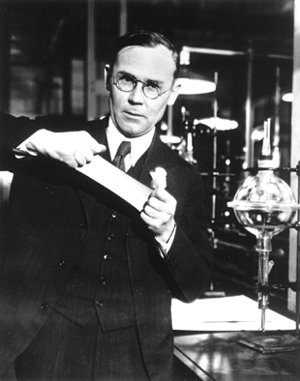
\includegraphics[width=0.24\linewidth]{images/book1/carothers.jpg}

{\small Wallace Carothers in his laboratory.}
\end{omfigure}

\section{Structure and properties}

Two samples of the same \omterm{def:g12:polymers:polymer}{polymer} can behave very differently: what
counts is the length of the chains, their shape, and how they are packed.

\begin{proposition}[Chains and properties]\label{prop:g12:polymers:properties}
\begin{itemize}
  \item Longer chains tangle more: the material is stronger and melts at
        a higher temperature.
  \item Linear chains can line up side by side in ordered,
        \emph{crystalline} regions; branched chains cannot, and stay
        disordered, \emph{amorphous}. Crystalline regions make a
        \omterm{def:g12:polymers:polymer}{polymer} denser, stiffer and less transparent.
  \item Chains held side by side only by intermolecular forces slide past
        each other when heated: the \omterm{def:g12:polymers:polymer}{polymer} is a \omterm{def:g8:plastics:thermoplastic}{thermoplastic}. Chains
        joined by covalent \emph{cross-links} cannot: the \omterm{def:g12:polymers:polymer}{polymer} is a
        \omterm{def:g8:plastics:thermoplastic}{thermoset}, or, with few cross-links, a rubber-like elastic
        solid.
\end{itemize}
\end{proposition}

\begin{proof}
Heating gives the chains enough energy to overcome the intermolecular
forces between them (\cref{ch:g11:polarity-and-cohesion}), which are
weaker than \omterm{def:g10:lewis-and-shape:covalent-bond}{covalent bonds}; the more contact between chains, the more
energy this takes. Cross-links are covalent: breaking them destroys the
material instead of melting it.
\end{proof}

\begin{omfigure}
\begin{tikzpicture}[font=\footnotesize, line width=1pt, line cap=round,
    lab/.style={below, align=center, text width=2.8cm}]
  % linear, packed (crystalline)
  \begin{scope}
    \foreach \y in {0,0.25,0.5,0.75,1.0}
      \draw[omDef] plot[smooth, domain=0:2.2, samples=25] (\x, {\y + 0.05*sin(400*\x)});
    \node[lab] at (1.1,-0.2) {linear chains\\ lined up: crystalline};
  \end{scope}
  % linear, tangled (amorphous)
  \begin{scope}[xshift=3.4cm]
    \draw[omDef] plot[smooth] coordinates {(0,0.2) (0.5,0.9) (1.0,0.3) (1.4,1.1) (2.0,0.5) (2.2,0.9)};
    \draw[omProp] plot[smooth] coordinates {(0,0.9) (0.4,0.3) (0.9,1.0) (1.5,0.2) (1.9,1.0) (2.2,0.3)};
    \draw[black!60] plot[smooth] coordinates {(0.1,0.55) (0.7,0.1) (1.2,0.75) (1.7,0.55) (2.2,0.1)};
    \node[lab] at (1.1,-0.2) {linear chains\\ tangled: amorphous};
  \end{scope}
  % branched
  \begin{scope}[xshift=6.8cm]
    \draw[omDef] plot[smooth] coordinates {(0,0.5) (0.6,0.6) (1.2,0.45) (1.8,0.65) (2.2,0.5)};
    \draw[omDef] (0.5,0.6) -- (0.35,1.05) (1.0,0.5) -- (1.15,0.05) (1.6,0.6) -- (1.5,1.1) (1.6,0.6) -- (1.95,1.0);
    \node[lab] at (1.1,-0.2) {branched chains:\\ cannot pack};
  \end{scope}
  % cross-linked
  \begin{scope}[xshift=10.2cm]
    \foreach \y in {0.1,0.55,1.0}
      \draw[omDef] plot[smooth, domain=0:2.2, samples=25] (\x, {\y + 0.06*sin(300*\x)});
    \foreach \x/\a/\b in {0.4/0.1/0.55, 1.3/0.1/0.55, 0.9/0.55/1.0, 1.9/0.55/1.0}
      \draw[omProp, line width=1.6pt] (\x,\a) -- (\x,\b);
    \node[lab] at (1.1,-0.2) {chains cross-linked:\\ do not melt};
  \end{scope}
\end{tikzpicture}

{\small Four arrangements of \omterm{def:g12:polymers:polymer}{polymer} chains. The cross-links (orange) are
\omterm{def:g10:lewis-and-shape:covalent-bond}{covalent bonds} between chains.}
\end{omfigure}

\begin{example}[Two polyethenes]\label{ex:g12:polymers:two-pe}
Polyethene made under very high pressure has many short branches: its
chains pack badly, and it gives soft, transparent films for bags. Made
with a \omterm{def:g12:catalysis:catalyst}{catalyst} at low pressure, its chains are nearly linear and pack
into crystalline regions: it is denser and stiffer, and gives milk
bottles and crates. Same \omterm{def:g12:polymers:polymer}{monomer}, same \omterm{def:g12:polymers:repeat-unit}{repeat unit}, different
architecture.
\end{example}

\section{Natural polymers}

Living things made \omterm{def:g12:polymers:polymer}{polymers} long before chemists did.

\begin{itemize}
  \item \textbf{Cellulose} and \textbf{starch} are both chains of glucose
        units, \ce{C6H10O5} per unit, joined differently: cellulose
        forms straight, strong fibres (wood, cotton, paper); starch forms
        coils that the body digests.
  \item \textbf{Proteins} are chains of amino acids joined by \omterm{def:g11:functional-groups:amine}{amide} links,
        the peptide bonds of the dipeptide of
        \cref{ch:g12:synthesis-strategy}.
  \item \textbf{DNA} is a chain of nucleotides; the order of its four
        kinds of unit stores genetic information.
  \item \textbf{Natural rubber} is an \omterm{def:g12:polymers:addition-polymer}{addition polymer} of isoprene,
        \ce{CH2=C(CH3)-CH=CH2}, collected as a milky liquid, latex, from
        the bark of the rubber tree. Heated with sulfur, its chains are
        linked by sulfur bridges: the rubber becomes tougher and keeps its
        shape, as in a tyre.
\end{itemize}

\begin{omfigure}
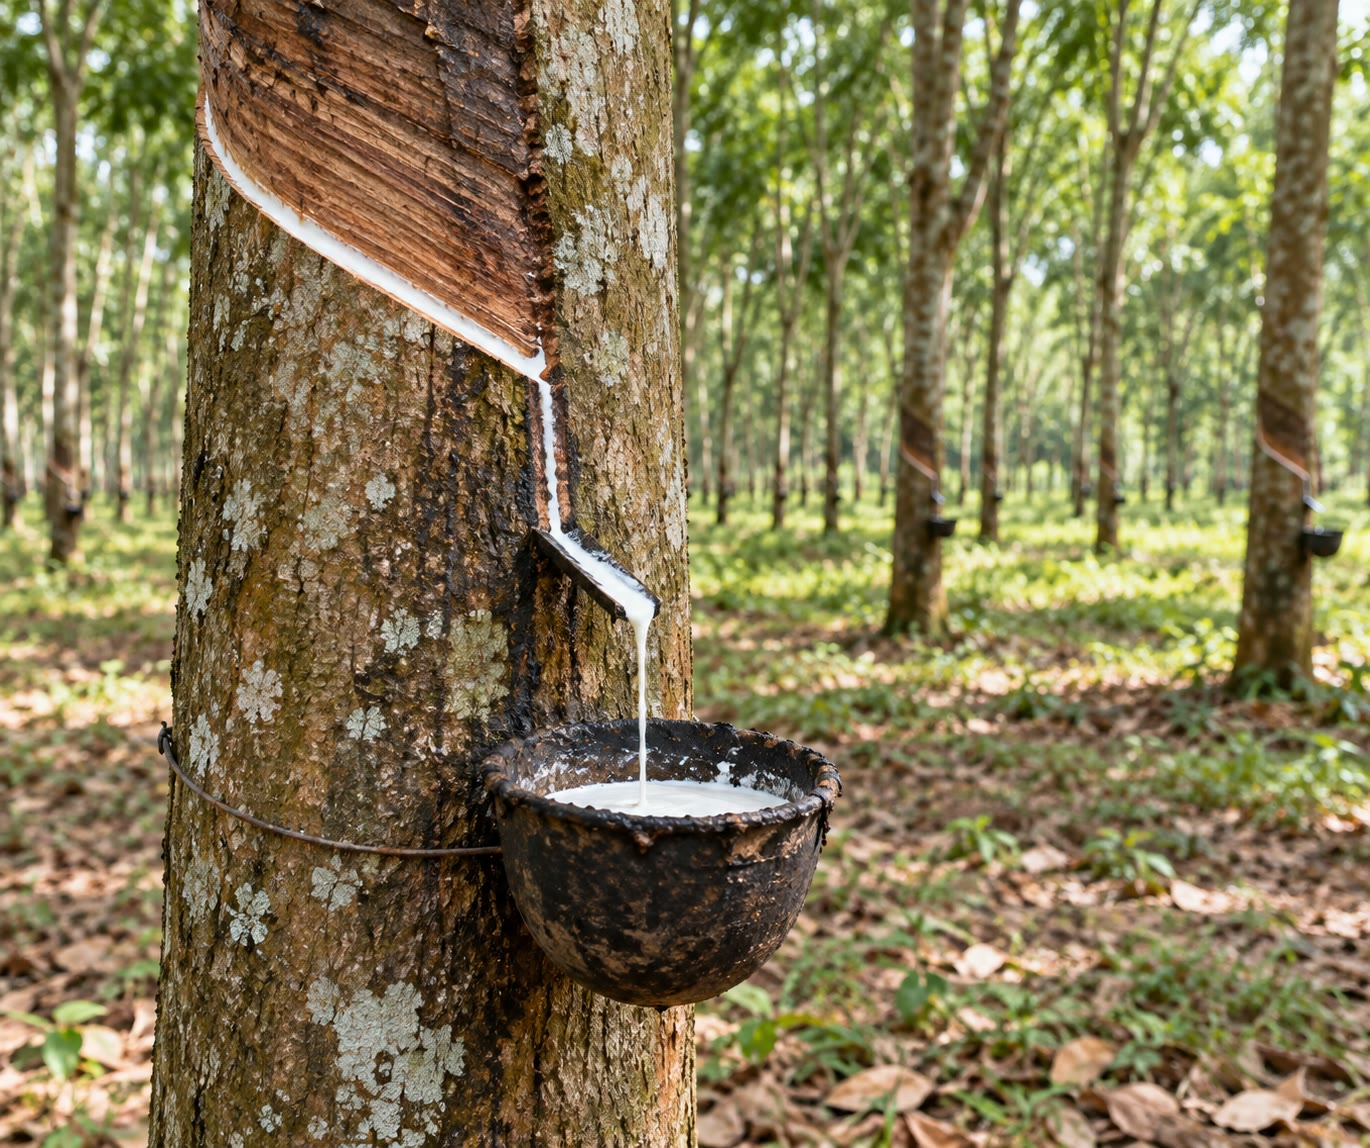
\includegraphics[width=0.45\linewidth]{images/book1/ai/g12-rubber-tapping.jpg}

{\small Tapping a rubber tree: latex flows from a cut in the bark into a
cup.}
\end{omfigure}

\begin{remark}[Making and unmaking]\label{rem:g12:polymers:recycling}
A \omterm{def:g8:plastics:thermoplastic}{thermoplastic} can be melted and shaped again: mechanical \omterm{def:g5:raw-materials-and-recycling:recycling}{recycling}. A
\omterm{def:g12:polymers:addition-polymer}{condensation polymer} can also be broken down to its \omterm{def:g12:polymers:polymer}{monomers} by the
reverse reaction, a hydrolysis, and the \omterm{def:g12:polymers:polymer}{monomers} made into new \omterm{def:g12:polymers:polymer}{polymer}:
chemical \omterm{def:g5:raw-materials-and-recycling:recycling}{recycling}. A \omterm{def:g8:plastics:thermoplastic}{thermoset} can do neither easily.
\end{remark}

\section{Exercises}

\begin{exercise}[$\star$]\label{exo:g12:polymers:1}
Give the \omterm{def:g12:polymers:polymer}{monomer} of polypropene, whose \omterm{def:g12:polymers:repeat-unit}{repeat unit} is
\ce{-CH2-CH(CH3)-}.
\end{exercise}

\begin{exercise}[$\star$]\label{exo:g12:polymers:2}
Write the \omterm{def:g12:polymers:repeat-unit}{repeat unit} of the \omterm{def:g12:polymers:polymer}{polymer} made from tetrafluoroethene,
\ce{CF2=CF2}. Is it an addition or a \omterm{def:g12:polymers:addition-polymer}{condensation polymer}?
\end{exercise}

\begin{exercise}[$\star$]\label{exo:g12:polymers:3}
Classify as addition or \omterm{def:g12:polymers:addition-polymer}{condensation polymers}: polyethene, PET, nylon,
PVC, polystyrene.
\end{exercise}

\begin{exercise}[$\star$]\label{exo:g12:polymers:4}
Which of these \omterm{def:g12:polymers:polymer}{polymers} are natural: cellulose, nylon, starch, PVC,
rubber from latex, proteins?
\end{exercise}

\begin{exercise}[$\star$]\label{exo:g12:polymers:5}
Why must each \omterm{def:g12:polymers:polymer}{monomer} of a \omterm{def:g12:polymers:addition-polymer}{condensation polymer} carry two reactive
groups?
\end{exercise}

\begin{exercise}[$\star\star$]\label{exo:g12:polymers:6}
A sample of PVC has an average \omterm{def:g10:the-mole:molar-mass}{molar mass} of \qty{125000}{g/mol}.
Compute its \omterm{def:g12:polymers:repeat-unit}{degree of polymerisation}.
\end{exercise}

\begin{exercise}[$\star\star$]\label{exo:g12:polymers:7}
A chain of polystyrene has a \omterm{def:g12:polymers:repeat-unit}{degree of polymerisation} of 2500. Compute
its \omterm{def:g10:the-mole:molar-mass}{molar mass}.
\end{exercise}

\begin{exercise}[$\star\star$]\label{exo:g12:polymers:8}
Lactic acid, \ce{CH3-CH(OH)-COOH}, carries an \omterm{def:g11:functional-groups:alcohol}{alcohol} group and an acid
group. Show that it can form a polyester on its own, write its \omterm{def:g12:polymers:repeat-unit}{repeat
unit}, and name the small \omterm{def:g7:atoms-and-molecules:molecule}{molecule} released.
\end{exercise}

\begin{exercise}[$\star\star$]\label{exo:g12:polymers:9}
Explain, with the figure of chain arrangements, why bag films are soft
and transparent while milk bottles are stiff and opaque.
\end{exercise}

\begin{exercise}[$\star\star$]\label{exo:g12:polymers:10}
The handle of a pan is a \omterm{def:g8:plastics:thermoplastic}{thermoset}, its \omterm{def:g8:plastics:plastic}{plastic} lid knob too. Describe
their chains. Why can they not be melted and recycled?
\end{exercise}

\begin{exercise}[$\star\star$]\label{exo:g12:polymers:11}
A chain of nylon-6,6 has a \omterm{def:g10:the-mole:molar-mass}{molar mass} of \qty{22600}{g/mol}. Compute the
\omterm{def:g10:the-mole:molar-mass}{molar mass} of its \omterm{def:g12:polymers:repeat-unit}{repeat unit} \ce{C12H22N2O2}, then its \omterm{def:g12:polymers:repeat-unit}{degree of
polymerisation}.
\end{exercise}

\begin{exercise}[$\star\star\star$]\label{exo:g12:polymers:12}
Write the reaction between one \omterm{def:g7:atoms-and-molecules:molecule}{molecule} of hexane-1,6-diamine and one of
hexanedioic acid, giving the first \omterm{def:g11:functional-groups:amine}{amide} link. Why can the product go on
reacting at both ends?
\end{exercise}

\begin{exercise}[$\star\star\star$]\label{exo:g12:polymers:13}
What mass of water is released when \qty{1.0}{kg} of nylon-6,6 is made?
\end{exercise}

\begin{exercise}[$\star\star\star$]\label{exo:g12:polymers:14}
Natural rubber is soft and sticky when warm; heated with sulfur, it
becomes the elastic, tough rubber of tyres. Explain with the chains.
Why is a tyre so hard to recycle?
\end{exercise}

\begin{exercise}[$\star\star\star$]\label{exo:g12:polymers:15}
Starch and cellulose have the same formula per unit, \ce{C6H10O5}. A
cellulose chain has a \omterm{def:g10:the-mole:molar-mass}{molar mass} of \qty{1.6e6}{g/mol}. How many glucose
units does it hold? How long is it, if each unit adds \qty{0.5}{nm} to
its length?
\end{exercise}

\section{Problem: From Bottle to Fleece}

\begin{problem}[{Weekend problem --- how many 25 g bottles go into one
fleece jacket?}]
\label{pb:g12:polymers:1}
% ledger: aw:C, aw:H, aw:O
A fleece jacket is made of \qty{300}{g} of PET fibre. Used bottles of
\qty{25}{g} each are collected, sorted, washed, shredded, melted and spun;
in this process \qty{80}{\percent} of the mass of the bottles ends up as
fibre in the jacket.

\medskip
\noindent\textbf{Part I --- The \omterm{def:g12:polymers:polymer}{polymer}.}
\begin{enumerate}
  \item Name the two \omterm{def:g12:polymers:polymer}{monomers} of PET and the \omterm{def:g11:functional-groups:functional-group}{functional groups} they
        carry.
  \item Which link forms between them? What small \omterm{def:g7:atoms-and-molecules:molecule}{molecule} is released?
  \item Is PET an addition or a \omterm{def:g12:polymers:addition-polymer}{condensation polymer}?
  \item Compute the molar masses of the two \omterm{def:g12:polymers:polymer}{monomers}.
  \item Deduce the \omterm{def:g10:the-mole:molar-mass}{molar mass} of the \omterm{def:g12:polymers:repeat-unit}{repeat unit} \ce{C10H8O4}, and check
        it with its formula.
\end{enumerate}

\medskip
\noindent\textbf{Part II --- The chains.}
\begin{enumerate}[resume]
  \item The PET of a bottle has chains of average \omterm{def:g10:the-mole:molar-mass}{molar mass}
        \qty{38400}{g/mol}. Compute the \omterm{def:g12:polymers:repeat-unit}{degree of polymerisation}.
  \item How many \omterm{def:g11:functional-groups:carboxylic-acid}{ester} links does one chain contain, about?
  \item PET of bottles is partly crystalline. What does that say about
        its chains?
  \item Why can PET be melted and spun into a fibre?
\end{enumerate}

\medskip
\noindent\textbf{Part III --- \omterm{def:g5:raw-materials-and-recycling:recycling}{Recycling}.}
\begin{enumerate}[resume]
  \item What mass of bottles is needed for one jacket?
  \item How many bottles is that?
  \item What happens to the rest of the mass?
  \item Which principle of \omterm{def:g12:synthesis-strategy:green-chemistry}{green chemistry} does this \omterm{def:g5:raw-materials-and-recycling:recycling}{recycling} apply?
\end{enumerate}

\medskip
\noindent\textbf{Part IV --- Back to the \omterm{def:g12:polymers:polymer}{monomers}.}
\begin{enumerate}[resume]
  \item Write, for one \omterm{def:g12:polymers:repeat-unit}{repeat unit}, the hydrolysis of PET into its
        \omterm{def:g12:polymers:polymer}{monomers}.
  \item What amount of \omterm{def:g12:polymers:repeat-unit}{repeat units} is there in \qty{1.00}{kg} of PET?
  \item What masses of each \omterm{def:g12:polymers:polymer}{monomer} does the full hydrolysis of
        \qty{1.00}{kg} of PET give?
  \item What mass of water does it consume? Check the \omterm{def:g8:balanced-equations:conservation}{conservation of
        mass}.
  \item Give one advantage of this chemical \omterm{def:g5:raw-materials-and-recycling:recycling}{recycling} over melting.
  \item State the final answer: how many \qty{25}{g} bottles go into one
        fleece jacket?
\end{enumerate}
\end{problem}
